\chapter{Коллективная азимутальная анизотропия в столкновениях тяжелых ионов} \label{chapt1}

\section{Обзор литературы по анизотропии рожденных частиц в столкновенях тяжелых ионов}

Равновесные свойства сильновзаимодействующей материи выражаются в форме уравнения состояния (Equation of State — EoS). 
Уравнение состояния определяет взаимосвязь между макроскопическими характеристиками материи, такими как температура, плотность, вязкость, давление и другие.
В современных моделях сильновзаимодействующей материи, основанных на гидродинамическом или статистическом подходах, уравнение состояния играет ключевую роль.
Фазовое состояние сильно взаимодействующей материи зависит от температуры ($T$) и чистой барионной плотности ($\rho_B$) --- разницы плотностей барионов и антибарионов.
С ростом температуры, которая является мерой средней кинетической энергии частиц в ансамбле, происходит высвобождения кварковых степеней свободы адронов.
Поскольку единичный адрон обладает внутренней структурой и ненулевым объемом, с ростом плотности или числа частиц на единицу объема, может достигаться состояние, в котором отдельные адроны более не различимы.
Таким образом, КХД материя может обладать как минимум, двумя различимыми фазами: с преобладанием адронных и преобладанием кварковых степеней свободы.
Характер перехода между этими двумя фазами является одним из открытых вопросов в этой области физики.
В области нулевых барионных плотностей возможно выполнить прямые расчеты КХД на решетке, которые предсказывают плавный переход ("cross-over") из кварковой материи в адронную~\cite{Esumi:2022uas}.
Однако данные теоретические методы неприменимы в области с ненулевой барионной плотностью.


Макроскопические свойства КХД материи представляют интерес для космологии и астрофизики. 
Согласно современным представлениям, эпохе бариогенезиса предшествовало состояние горячей кварк-глюонной материей с около нулевой барионной плотностью ($\rho_B~0$), которое завершилось плавным cross-over переходом в состояние материи с преимущественно адронными степенями свободы~\cite{Esumi:2022uas}.
В то время как, сверхплотная КХД-материя ($~\rho_B ~ 5\rho_0$) образуется в ядрах нейтронных звёзд~\cite{Danielewicz:2002pu} и при слиянии двойных звёздных систем~\cite{Adamczewski-Musch:2019byl}.
Система, образованная при столкновении пары тяжелых ионов, так же может быть достаточно велика для использования статистических методов ее описания.
Поэтому можно говорить о возникновении сильно взаимодействующей материи в области перекрытия сталкивающихся ионов.
Столкновения тяжелых ионов --- единственный способ экспериментально достичь схожих состояний материи, образующейся в сложнонаблюдаемых космологических объектах.

Основные сложности изучения КХД-материи образованной в столкновения ядер, заключаются в экстремально малых объёмах созданного вещества ($~10^3 fm^3$) и экстремально коротких характерных временах его существования $~20fm/c$. 
Экспериментальные методы исследования столкновений тяжелых ионов ограничены измерением лишь конечного результата столкновений.
Экспериментально недоступными остаются параметры начального состояния системы: прицельный параметр, флуктуации плотности энергии, число нуклонов-участников столкновения, и т.д.
Начальное состояние системы может быть реконструировано при помощи статистического моделирования и сравнения теоретических предсказаний модели с измеренными экспериментально наблюдаемыми.
Статистические модели позволяют связать спектры рожденных частиц, их импульсное распределение с температурой достигнутой в системе в центральных столкновениях.
Однако данные модели оказываются несостоятельными в описании менее центральных и менее горячих столкновений~\cite{NA49:2004iqm, UA5:1981lmw}.

В 1955 году Ландау и Беленький~\cite{Belenkij:1955pgn} впервые применили подход вязкой гидродинамики для описания столкновений тяжелых ионов. 
В середине 1970-х годов было выдвинуто предположение что динамика столкновений подвержена влиянию "ударных волн", которые формируются при пересечении сталкивающихся ионов~\cite{Chapline:1973kkq}.
Шилд, Мюллер и Грайнер впервые обратили внимание на значимость расширения области перекрытия в направлении поперечном направлению пучка в работе~\cite{Scheid:1974zz}.
Авторы пришли к заключению, что образованная материя выталкивается перпендикулярно направлению движения сталкивающихся ионов. 
Эффекты коллективного движения частиц проявляются относительно плоскости симметрии, определенной направлением прицельного параметра $b$ и оси пучка $z$.
Эта плоскость получила название плоскости реакции и общепринятое обозначение $\Psi_{RP}$.

Эффект наличия у рожденных в столкновении частиц преимущественного направления вылета впервые был экспериментально обнаружен на установке Plastic Ball/Wall на Линейном ускорителе Беркли~\cite{Gustafsson:1984ka}. 
Ненулевой средний поперечный импульс рожденных частиц направлен в плоскости реакции, перпендикулярно изначальному движению сталкиваемых ионов.
Этот эффект получил название "бокового потока" (sideflow).
Изначально, боковой поток характеризовался как средняя $x$-компонента поперечного импульса частиц в плоскости реакции:
\begin{equation}
    \langle p_x \rangle = \frac{1}{N}{\sum_{k=1}^N p_x^k},
\end{equation}
где плоскость реакции ориентирована по направлению оси $x$.

Преобладание вылета рожденных частиц перпендикулярно плоскости реакции, вдоль оси $y$, впервые было зафиксировано на эксперименте Diogene в столкновениях с неоновым пучком при энергии $E_{kin}=800A$~МэВ~\cite{Demoulins:1990ac}.
В дальнейшем коллаборация Plastic Ball произвела систематическое исследование этого явления в столкновениях Au~+~Au при различных энергиях~\cite{Gustafsson:1984qh, Gutbrod:1988hh}.
Численно это было оценено как отношение числа частиц вылетевших перпендикулярно плоскости реакции к числу частиц в плоскости реакции:
\begin{equation}
    R_N = \frac{ N(90^{\circ} ) + N(-90^{\circ}) }{ N(0^{\circ}) + N(180^{\circ}) }
\end{equation}

В дальнейшем Волошин и Жанг~\cite{Voloshin:1994mz, Poskanzer:1998yz} предложили исследовать импульсную анизотропию рожденных частиц путём разложения азимутального распределения частиц в ряд Фурье:
%
\begin{equation}
    \frac{1}{p_T}\frac{d^3 N}{dp_T dy d\phi} = 
    \frac{ 1 }{2\pi p_T} \frac{ d^2 N }{dp_T dy} \{
    1 + 2\sum_{n=1}^{\infty} v_n(p_T,y) \cos[ n ( \phi - \Psi_R ) ]
    \},
\end{equation}
%
где $\phi$ --- азимутальный угол частицы, $\Psi_{RP}$ --- угол плоскости реакции, определенный вектором прицельного параметра и направлением пучка, $p_T$ --- поперечный импульс и $y$ --- быстрота частицы.
Коэффициенты разложения определяются как 
%
\begin{equation}
    v_n(p_T,y) = \langle  \cos[ n ( \phi - \Psi_R ) ] \rangle,
\end{equation}
%
где угловые скобки означают усреднение по всем частицам и всем событиям. 
Коэффициенты $v_1$ и $v_2$ носят названия направленного (directed) и эллиптического (elliptic) потоков.

Связывая исторические методы измерения с современными, мы получим, что боковой поток выражается через направленный поток следующим образом:
\begin{equation}
    \langle p_x \rangle = v_1 \langle p_T \rangle 
\end{equation},
где $\langle p_T \rangle $ --- средний поперечный импульс рожденных частиц.
Коэффициент $R_N$ зависит от $v_2$ согласно формуле:
\begin{equation}
    R_N = \frac{1 - v_2}{1 + v_2}.
\end{equation}
Новые методы измерения коллективной анизотропии рожденных частиц в связке с большей набираемой статистикой данных открывают возможность мультидифференциального исследования гармоник потока $v_n$, что позволяет производить более детальное сравнение с теоретическими моделями.

На рис.~\ref{fig:eos_px_y} показаны данные коллаборации EOS~\cite{EOS:1994kku} для среднего импульса частиц в плоскости реакции $\langle p_x /A \rangle$ как функция быстроты нормализованной на быстроту пучка $y/y_{beam}$ для столкновений Au~+~Au при энергии $E_{kin}=800A$~МэВ.
Изначальный поперечный импульс сталкивающихся нуклонов равен нулю и конечный импульс рожденных в столкновении частиц приобретён из-за коллективного расширения области перекрытия в плоскости реакции.
Поскольку расширение происходит симметрично, средний импульс является антисимметричной функцией быстроты $y/y_{beam}$.
%
\begin{figure}
    \centering
    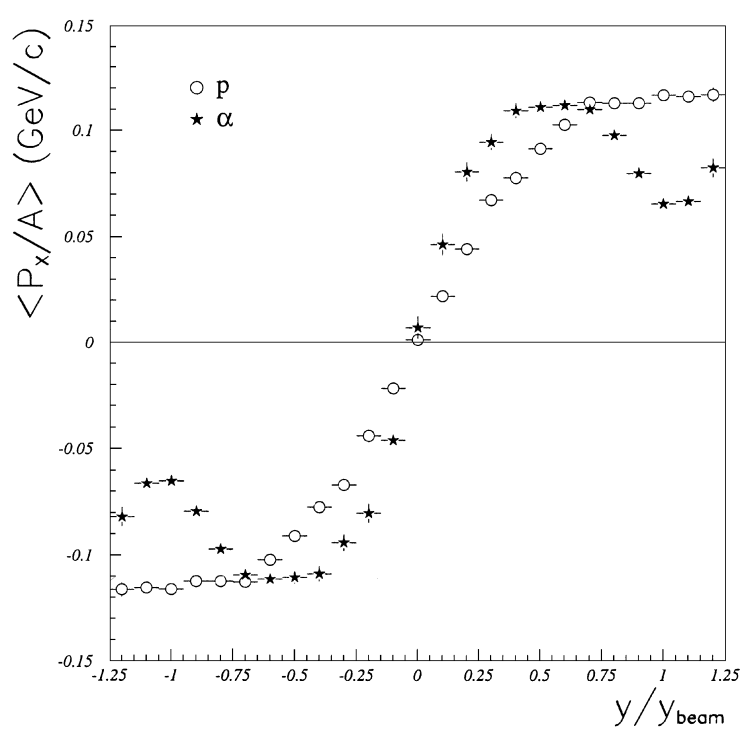
\includegraphics[width=0.55\linewidth]{images/eos_px_y.png}
    \caption{Средний импульс частиц в плоскости реакции $\langle p_x /A \rangle$ как функция быстроты нормализованной на быстроту пучка $y/y_{beam}$ для столкновений Au~+~Au при энергии $E_{kin}=800A$~МэВ. Данные коллаборации EOS~\cite{EOS:1994kku}.}
    \label{fig:eos_px_y}
\end{figure}

Функция среднего приобретённого импульса рожденных в столкновении частиц может быть охарактеризована наклоном в средних быстротах $F=d\langle p_x /A \rangle / dy|_{y=0}$.
На рис.~\ref{fig:F_pball} показан наклон $F$ как функция энергии столкновения для симметричных систем. 
Данные взяты из~\cite{Gutbrod:1989wd, EOS:1994kku, EOS:1996kon, FOPI:2011aa}
За исключением данных FOPI, наклон был вычислен при помощи частиц с зарядом 1 и 2.
$F$ возрастает как функция энергии столкновения до $E_{kin} \approx 250A$~МэВ.
Затем средний приобретенный импульс рожденных частиц начинает убывать после значений $E_{kin} \approx 400A$~МэВ.
Данные эксперимента FOPI получены для более тяжелых фрагментов и в 1.4 раза больше по сравнению с $F$, полученным для более лёгких частиц. 
Этот эффект может быть связан с коалесценцией лёгких фрагментов и воспроизводится в теоретических вычислениях~\cite{EOS:1994jzn}.
%
\begin{figure}
    \centering
    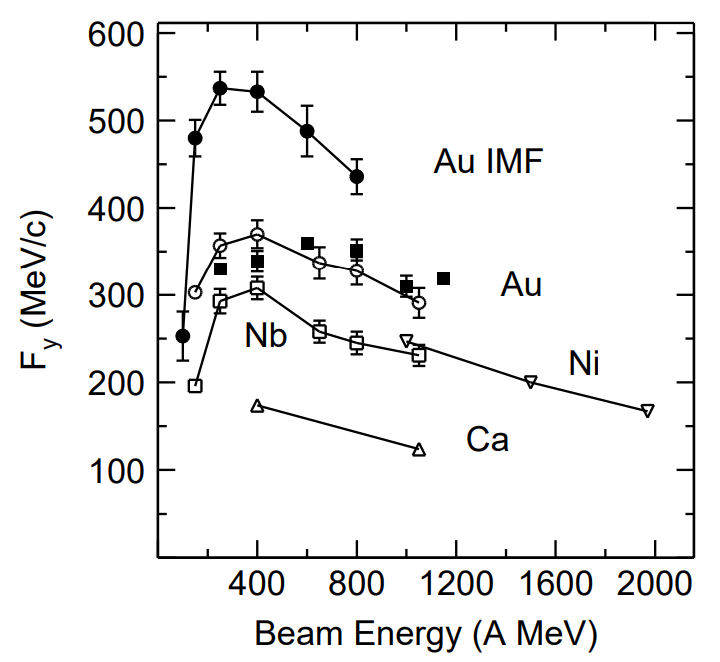
\includegraphics[width=0.55\linewidth]{images/F_energy.png}
    \caption{Наклон $F=d\langle p_x /A \rangle / dy|_{y=0}$ как функция энергии столкновения для симметричных систем. Данные взяты из~\cite{Gutbrod:1989wd, EOS:1994kku, EOS:1996kon, FOPI:2011aa}.}
    \label{fig:F_pball}
\end{figure}

В последующие годы экспериментальные измерения среднего импульса были выполнены на множестве экспериментальных установок (EOS, FOPI, E877, E917, E895, NA49 и WA98) в большом диапазоне энергий.
Коллаборация FOPI произвела систематическое исследование направленного и эллиптического потоков для 25 комбинаций систем (Ca+Ca, Ni+Ni, Xe+CsI, Ru+Ru, Zr+Zr, Au+Au) и энергий ($E_{kin}=0.09-1.5A$~ГэВ)~\cite{FOPI:2011aa}. 
На рис.~\ref{fig:FOPI_v11_energy} показана зависимость наклона направленного потока протонов $v_{11}$ от энергии столкновения ядер золота. 
Открытыми символами показаны значения $v_{11}$ для 4-скорости $u_{t0}>0.8$, заполненными --- для $u_{t0}>0.4$.
Наклон направленного потока довольно сильно зависит от выбора диапазона относительного прицельного параметра $b_0$.
Для среднецентральных столкновений ($0.25<b_0<0.45$) наклон направленного потока слабо зависит от энергии столкновения после $E_{kin}>0.5A$~ГэВ.

\begin{figure}
    \centering
    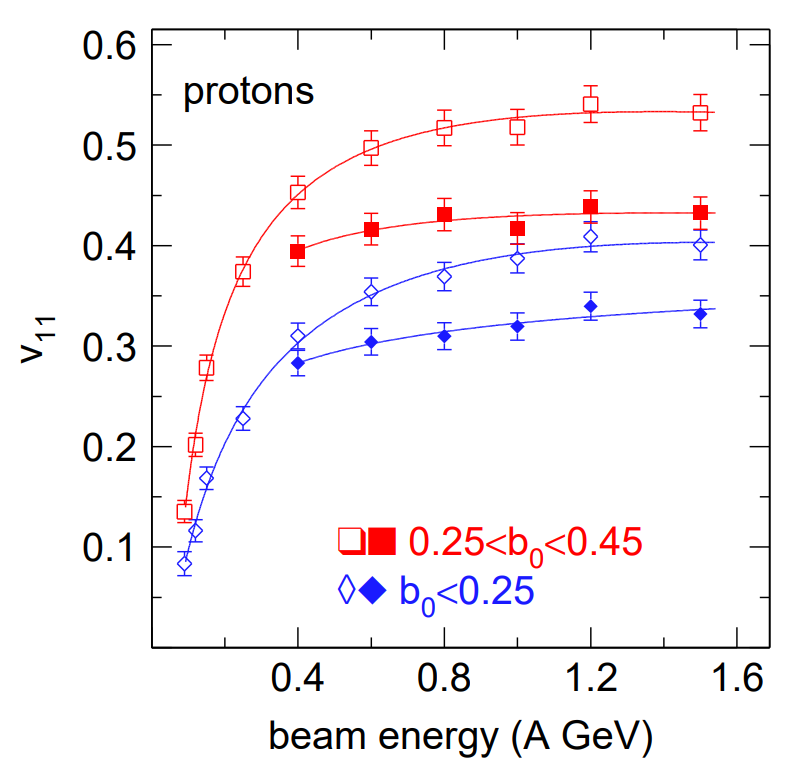
\includegraphics[width=0.5\linewidth]{images/FOPI_v11_energy.png}
    \caption{Зависимость наклона направленного потока протонов $v_{11}$ от энергии столкновения ядер золота. Открытыми символами показаны значения $v_{11}$ для 4-скорости $u_{t0}>0.8$, заполненными --- для $u_{t0}>0.4$. Данные взяты из~\cite{FOPI:2011aa}.}
    \label{fig:FOPI_v11_energy}
\end{figure}

На рис.~\ref{fig:Fy_summary} приведена экспериментальная зависимость $F_y$ от энергии столкновения~\cite{Herrmann:1999wu}.
Наблюдается резкое падение коллективного потока с ростом энергии.
Пунктирная линия описывает простое предположение зависимости наклона от времени пролёта сталкивающихся ядер:
%
\begin{equation}
    F(y) = P_{eff} \times S \times t_{pass},
\end{equation}
%
где $P_{eff}$ --- среднее эффективное давление, $S$ --- площадь эффективной расширяющейся поверхности и $t_{pass}$ --- время пролета.
Теоретическое предсказание построено на предположении, что действующая сила $P_{eff} \times S$ постоянна, а уменьшение передачи импульса происходит только из-за сокращения времени пролёта $t_{pass}$.
Эта гипотеза довольно хорошо описывает экспериментальные данные при высоких энергиях, однако не учитывает влияние спектаторов, которое существенно при низких.

\begin{figure}
    \centering
    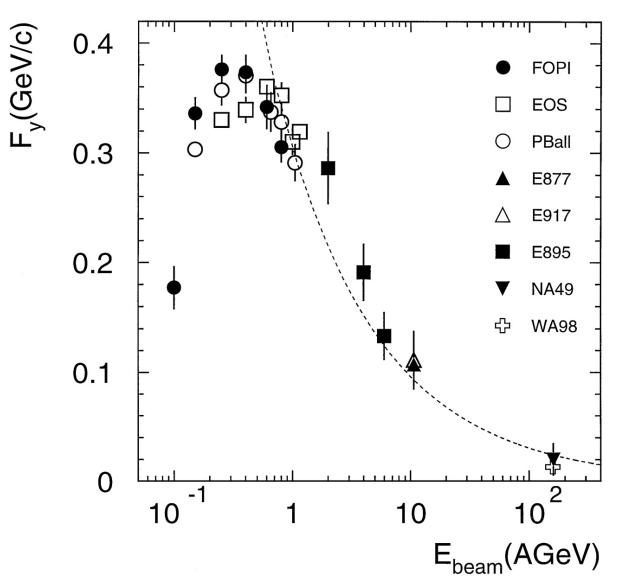
\includegraphics[width=0.55\linewidth]{images/Fy_summary.png}
    \caption{Наклон $F=d\langle p_x /A \rangle / dy|_{y=0}$ как функция энергии столкновения для симметричных систем~\cite{Herrmann:1999wu}.}
    \label{fig:Fy_summary}
\end{figure}

На рис.~\ref{fig:RN_energy} показана зависимость коэффициента $R_N$ от энергии столкновения для различных симметричных систем~\cite{Gustafsson:1984qh}.
Зависимость $R_N$ от энергии схожа с зависимостью $F_y$, показанной на рис.~\ref{fig:F_pball}. 
Данные для $R_N$ противоречат предсказаниям вязкой гидродинамики, согласно которым, потоки в разных системах должны быть схожи.

\section{Центральность столкновения}

В результате столкновения тяжелых ионов в области перекрытия образуется сильно взаимодействующая материя, свойства которой сильно зависят от размера сталкивающихся ядер, и от энергии столкновения.
При столкновении тяжелых ядер, при энергиях в несколько ГэВ на нуклон налетающего ядра, время пролёта ионов сравнимо со временем существования материи в области перекрытия.
Процесс столкновения двух ядер можно условно разделить на несколько этапов.

Начальная фаза определяет геометрию столкновения, а именно прицельный параметр $b$ --- расстояние между центрами сталкивающихся ядер, пространственное распределение нуклонов, число нуклонов-партисипантов, испытывающих в ходе столкновения неупругие рассеяния и число нуклонов-спектаторов, взаимодействующих лишь упруго.  
Экспериментальное измерение прицельного параметра невозможно, поэтому необходима физическая наблюдаемая, по которой можно судить о геометрии столкновения.
Этой наблюдаемой является центральность столкновения, как отношение сечения взаимодествия в данном диапазоне параметра $S=[S_1, S_2]$ к полному сечению неупругого взаимодействия:
%
\begin{equation}
    C_S = \frac{1}{ \sigma_{inel}^{AA} } \int_{S_1}^{S_2} \frac{d\sigma}{dS}dS,
\end{equation}
где $C_S$ --- центральность столкновения по выбранному эстиматору центральности $S$, $\sigma_{inel}^{AA}$ --- полное сечение неупругого взаимодействия двух ядер, $S_{1,2}$ --- границы класса центральности.
В качестве эстиматора класса центральности в эксперименте часто выбирается множественность частиц, либо величина пропорциональная ей.
При помощи модели Монте-Карло Глаубера~\cite{Miller:2007ri} разыгрываются геометрические параметры столкновения, такие как прицельный параметр $b$, число партисипантов $N_{part}$, число бинарных неупругих рассеяний $N_{col}$.
Используя отрицательное биномиальное распределение и выход Монте-Карло Глаубера моделирования подбирается множественность рожденых частиц, которая будет аппроксимировать эксеприментальное распределение множественности.
На основании этого затем определяются классы центральности и извлекаются средние значения геометрических параметров для каждого класса.

\section{Коллективные эффекты в столкновениях тяжелых ядер}

При скоростях налетающего ядра, превышающих скорость звука в ядерной материи при при обычных условиях ($\beta_S=0.2$)~\cite{Weber:1998aa}, нуклоны не могут покинуть область перекрытия достаточно быстро, и образуется зона высокой плотности.
В зависимости от уравнения состояния, которое связывает давление с плотностью и температурой, материя в зоне перекрытия может достигать условий, которые описываются средней плотностью и температурой.
В этих условиях могут быть созданы новые частицы, а их число и характер эмиссии могут быть использованы для исследования глобальных свойств вещества.
Отклонение плотным веществом в области перекрытия, остатков налетающего ядра с положительной быстротой происходит в направлении $+x$, что приводит к $\langle p_x \rangle  > 0$, а остатки ядра с отрицательной быстротой отклоняются в направлении $-x$, таким образом, имея $\langle p_x \rangle < 0$.
Таким образом, направленный поток остатков налетающего ядра является положительным для частиц с положительной бысротой и отрицательным для частиц с отрицательной быстротой.
Измерения направленного потока частиц, относительно плоскости симметрии определенной спектаторами даёт информацию о времени взаимодействия рожденных частиц с областью перекрытия.
Положительный направленный поток частиц относительно плоскости симметрии остатков налетающего ядра говорит о довольно большом времени взаимодействия, при котором материя в области перекрытия успевает смешаться с холодной спектаторной материей.
Эллиптический поток $v_2$ несёт информацию о давлении в области перектия сталкивающихся ионов.
При энергиях порядка 1~ГэВ, значения $v_2$ отрицательные относительно плоскости симметрии спектаторов.
Остатки сталкивающихся ядер блокируют вылет частиц в плоскости реакции, что ведет к вылету частиц перпендикулярно плоскости реакции.
Чем выше давление, достигаемое в области перекрытия, тем выше будут значения $v_2$.
Схематически эти механизмы изображены на рис.~\ref{fig:bounce_off}.
%
\begin{figure}[ht]
\begin{center}
    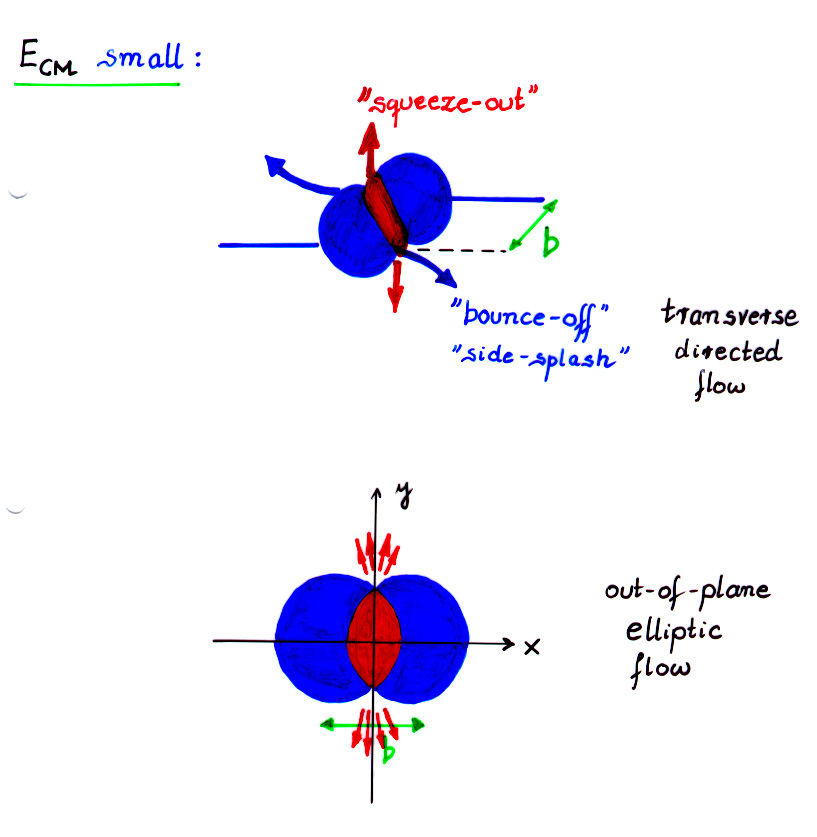
\includegraphics[width=0.75\linewidth]{images/bounce_off.jpg}
    \caption{Схематичное изображение механизмов рождения направленного (bounce-off) эллиптического (squeeze-out) потоков.}
    \label{fig:bounce_off}
\end{center}
\end{figure}
%

Партисипанты, или нуклоны сталкиващихся ядер, претерпевают многократные рассеяния.
В результате рождаются новые частицы и изменяются импульсы частиц, составляющих материю в области перекрытия.
Если время взаимодействия достаточно велико, то материю в области перекрытия можно описать при помощи статистических величин: средняя плотность, средняя температура и т.д..
При многократном рассеянии частиц, составляющих материю в области перекрытия, может происходить подпороговое рождение частиц.
Сравнивая коллективные потоки различных типов частиц, рожденных в области перекрытия можно судить о степени термализации или релаксации энергии в области перекрытия.
Чем ближе потоки различных типов сталкивающихся частиц к среднему значению, тем больше степень термализации материи.
По степени термализации можно судить о времени существования материии в области перекрытия.  

Реакция и развитие коллективных эффектов останавливаются на стадии столкновения, обычно называемой фриз-аут. 
В этой фазе плотности достаточно малы, чтобы в течение типичной длины пролета больше не происходило взаимодействия.
Хотя многие наблюдаемые (например, спектры рожденных частиц) теряют память о начальных условиях во время процесса эволюции, ожидается, что коллективные потоки адронов несут информацию о самых ранних этапах эволюции~\cite{Herrmann:1999wu}.
Коллективные потоки рожденных в столкновении адронов сильно зависят от начальной геометрии столкновения.
Коллективное движение рожденых адронов обусловлено взаимодействием частиц составляющих материю в области перекрытия.
Характер этого взаимодействия обусловлен свойствами материи, которые описываются уравнением состояния.
Поэтому зная изначальную геометрию столкновения, которая определяется центральностью и измеряя итоговую анизотропию рожденных частиц можно извлечь уравнение состояния сильновзаимодействующей материи.

Коллективное движение частиц приводит к корреляции импульсов рожденных адронов.
Таким образом, изучая эту корреляцию, можно количественно оценить коллективные эффекты.
Однако это не единственный канал, по которому импульсы рожденных частиц могут быть скоррелированы.
К примеру, импульсы частиц, рожденных в слабом или сильном распаде резонанса относятся следующим образом:
%
\begin{equation}
    P = P_1 + P_2,
\end{equation}
где $P$ --- 4-импульс резонанса, $P_{1,2}$ --- импульсы рожденных в распаде частиц.
Также в силу сохранения поперечного (полного) импульса системы справедливо следующее соотношение:
%
\begin{equation}
    \sum_{k=1}^{N} \vec{p_T}^k = 0,
\end{equation}
где $N$ --- множественность рожденных частиц, $\vec{p_{T}}^k$ --- поперечный импульс $k$-й частицы.
Корреляция импульсов частиц, рожденной в бинарном столкновении частиц, составляющих материю тоже подчиняется законам сохранения импульса:
%
\begin{equation}
    P_1 + P_2 = P_3 + P_4 + P_5.
\end{equation}

Описанные выше эффекты не имеют отношения к коллективному движению частиц, однако обеспечивают корреляцию импульсов.
Такие эффекты носят название непотоковых корреляций и осложняют измерение коллективных эффектов.
Поэтому для подавления непотоковых эффектов чаще всего рассматривается корреляция большого колличества частиц.
Также для подавления корреляций не связанных с коллективным движением частиц можно рассматривать корреляцию областей со значительнми разделением по кинематике.
Оценка вклада остаточных непотоковых корреляций является важной задачей при измерении коллективных эффектов.

\section{Основыне определения}

Методы измерения коллективных потоков довольно просто описать в терминах векторов.
Для измерения азимутальных потоков каждой частице ставится в соответствие единичный вектор $u_n$ в плоскости перпендикулярной оси пучка на основании импульса частицы:
%
\begin{equation}
    \vec{u_n} = (x_n, y_n) = ( \cos n \varphi, \sin n \varphi ),
\end{equation}
%
где $\varphi$ --- азимутальный угол частицы, $n$ --- порядок гармоники. 
При очень большом количестве частиц в одном событии ($N \gg 1$), сумму по всем частицам можно заменить на интеграл:
%
\begin{equation}
    \langle \vec{u_n} \rangle = \sum_{k=1}^{N} u_n = \int_{-\pi}^{\pi} \vec{u_n}(\phi) \rho(\phi-\Psi^R) d\phi
\end{equation}
Рассмотрим интеграл по $x$-компоненте $u_n$ вектора:
%
\begin{equation}
    \int_{-\pi}^{\pi} x_n \rho[n(\phi-\Psi^R)] d\phi =
    \int_{-\pi}^{\pi} \cos n ( \phi - \Psi^R + \Psi^R ) \rho[n(\phi - \Psi^R)] = V_n \cos (n\Psi^R), 
\end{equation}
где $V_n$ пропорционален множественности частиц $N$ и значению $v_n$ для данной группы частиц в данном событии.
Аналогичные преобразования можно выполнить и для $y$-компоненты $u_n$-вектора, получив $V_n\sin(n\Psi^R)$.
Таким образом, сумма $u_n$-векторов в одном событии даёт оценку плоскости реакции события.

Эта оцнека, определяемая суммой единичных векторов частиц носит название $Q_n$-вектора:
%
\begin{equation}
    \vec{Q_n} = \frac{1}{C} \sum_{k=1}^{N} w_k u_n^k = \frac{|Q_n|}{C} (\cos{(n\Psi_n)}, \sin{(n\Psi_n)}),
\end{equation}
%
где $k$ --- индекс частицы в группе, $w_k$ --- вес $k$-го вектора, $N$ --- множественность частиц в группе, $\Psi_n$ --- угол плоскости симметрии данного события и данной гармоники $n$, $|Q_n|$ --- модуь $Q_n$-вектора и $C$ --- нормировочный коэффициент. 
Чем больше число частиц в событии $N$, тем ближе оценка угла плоскости симметрии к реальной ориентации плоскости реакции:
%
\begin{equation}
    \lim_{N \xrightarrow{} \infty} \frac{1}{C} \sum_{k=1}^{N} w_k u_n^k = \frac{|Q_n|}{C} (\cos{n(\Psi^R)}}, \sin{n(\Psi^R)}) .
\end{equation}

\section{Методы плоскости события и скалярного произведеления}

Выбор значения нормировочного коэффициента определяет метод измерения направленного потока. 
В работе исследуются два метода: плоскости события (EP) и скалярного произведения (SP)~\cite{Mamaev:2020lpi}. 

Метод плоскости события (EP) требует такую нормировку, чтобы модуль каждого $Q_1$-вектора был равен 1, что соответствует $C=|Q_n|$. 
В работах~\cite{Borghini:2001vi, Bhalerao:2006tp} было показано, что в таком случае, измеренное значение потока $v_n\{EP\}$ нелинейно зависит от множественности частиц, использованных для вычисления $Q_n$-вектора, а также от значения самого потока. 
В пределе большого количества частиц и большого значения потока ($v_n \sqrt{M} \gg 1$), измеренные значения стремятся к среднему значению $v_n$: $v_n\{EP\} \xrightarrow{} \langle v_n \rangle$. 
В случае малого числа частиц, использованных для построения $Q_n$-вектора, а также малых значениях потока ($v_n \sqrt{M} \ll 1$), измерения стремятся к корню среднего квадрата $ v_n\{EP\} \xrightarrow{} \sqrt{ \langle v_n^2 \rangle }$.
Экспериментально измеренные значения $v_1\{EP\}$ находятся между двумя пределами: $ \langle v_n \rangle \leq v_n\{EP\} \leq \sqrt{ \langle v_n^2 \rangle } $.
В зависимости от реального значения $v_n$ (который определяется энергией столкновения и размером сталкивающихся ядер) и множественности частиц (которая зависит от энергии, размера ядер и аксептанса установки), измеренные значения $v_n\{EP\}$ могут лежать ближе к правому или левому пределам.

Второй метод, скалярного произведения (SP), требует нормировку на сумму весов $C=\sum_{k=1}^N w_k$.
Модуль $Q_n$-вектора сохраняет информацию о множественности частиц, использованных для его построения, а также их $v_n$: $|Q_n| \propto v_n M$.
Использование такой нормировки дает значения $v_n\{SP\} \xrightarrow{} \sqrt{\langle v_n^2 \rangle}$ независимо от измеренной множественности частиц, а также их $v_n$.

Несмотря на известные недостатки метода плоскости события, он до сих пор активно используется, поскольку более прост в реализации. 
В частности, измерения коэффициентов коллективных потоков $v_n$ в коллаборации HADES~\cite{HADES:2020lob} были выполнены методом плоскости события. 
В работе была произведена оценка систематической ошибки на измереные $v_n$, путём сравнения результатов полученных методами скалярного произведения и плоскости события~\cite{Mamaev:2020lpi}.

\section{Разрешение плоскости симметрии}

Экспериментально направленный поток можно определить как проекцию $u_n$-вектора частиц на плоскость симметрии события:
%
\begin{equation}
    v_n' =  \langle u_n Q_n \rangle = 
    V_n \langle \cos (n\phi) \cos (n\Psi_n) \rangle + V_n \langle \sin(n\phi) \sin(n\Psi_n) \rangle,
\end{equation}
%
где диагональные члены равны нулю в силу симметрии столкновения, а коэффициент $V_n$ появляется в силу усреднения модулей вектора $Q_n$.
Раскрывая тригонометрические выражения в угловых скобках, можно получить:
%
\begin{equation}
\begin{align}
    \langle \cos (n\phi) \cos (n\Psi_n) \rangle = \langle \cos n ( \phi - \Psi_n ) \rangle = \\
    = \langle \cos n ( \phi - \Psi_n + \Psi^R - \Psi^R ) \rangle =
    \langle \cos n ( \phi - \Psi^R ) \cos n (\Psi_n - \Psi^R ) \rangle
\end{align}
\end{equation}
%
Аналогичные преобразования можно выполнить и для синусов. 
Измеренные значения направленного потока имеют вид:
%
\begin{equation}
    v_n' =  \langle u_n Q_n \rangle = 
    V_n \langle \cos n ( \phi - \Psi_n ) \cos n (\Psi_n - \Psi^R) \rangle.
    \label{eq:uq_transformation}
\end{equation}
%

Поскольку вычисленная плоскость симметрии столкновения $\Psi_n$ лишь приблизительно описывает ориентацию плоскости реакции $\Psi^R$, значение $ \langle \cos(\Psi_n - \Psi^R) \rangle \ne 1 $.
Флуктуации распределения энергии в сталкивающихся ядрах приводят к флуктуации плоскости симметрии относительно плоскости реакции реакции, как показано на рис.~\ref{fig:pp_sp_rp}
Поэтому измеренные значения $v_n'$ будут отличаться от действительных.
Для коррекции этого этого эффекта, необходимо ввести поправочный коэффициент разрешения:
%
\begin{equation}
    R_n = V_n \langle \cos n (\Psi_n - \Psi^R) \rangle.
\end{equation}
%

%
\begin{figure}[ht]
\begin{center}
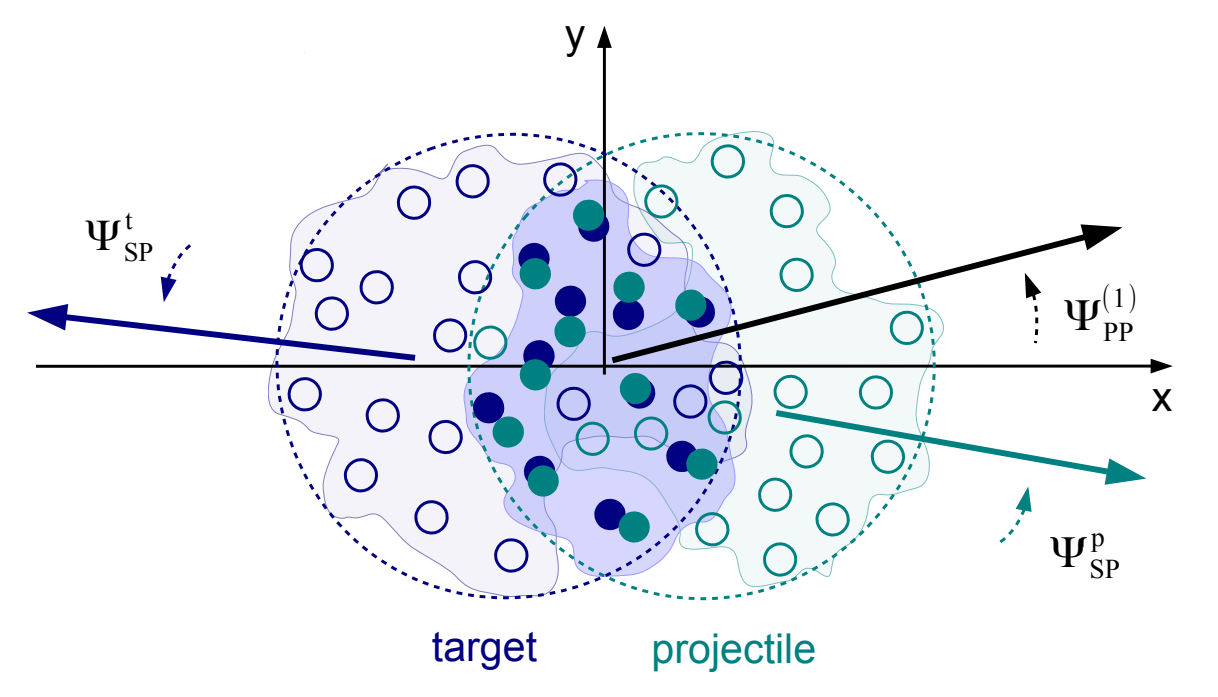
\includegraphics[width=0.75\linewidth]{images/v1_pp_sp.png}
\caption{Схематическое представление сталкивающихся ядера в плоскости перпендикулярной направлению пучка.}
\label{fig:pp_sp_rp}
\end{center}
\end{figure}
%

Скорректированные на разрешение значения $v_1$ могут быть записаны следующим образом: 
%
\begin{equation}
    v_n =  \frac{ \langle u_n Q_n \rangle }{R_n},
    \label{eq:v1_formula}
\end{equation}
%

\section{Метод случайных подсобытий}

Для вычисления $R_n$ в эксперименте, можно воспользоваться попарными корреляциями $Q_n$-векторов (преобразование выполнено аналогично уравнению (\ref{eq:uq_transformation})): 
%
\begin{equation}
    \langle Q_n^a Q_n^b \rangle = V^a_n V^b_n \langle \cos n (\Psi^a_n - \Psi^R) \cos(\Psi^b_n - \Psi^R) \rangle,
\end{equation}
%
где индексами $a$ и $b$ обозначены две различных группы частиц, в каждой из которых $Q_n$-вектор вычислялся независимо.

Наиболее простым методом вычисления разрешения является метод двух подсобытий:
%
\begin{equation}
    R_n\{a,b\} = \sqrt{ \langle Q_n^a Q_n^b \rangle } = \sqrt{ V_n^2 \langle \cos^{2}( \Psi^{a,b}_n - \Psi_R ) \rangle },
\end{equation}
где индексами $a$ и $b$ обозначены две группы частиц, идентичные по множественности и значению $v_n$, в которых $Q_n$-вектор вычислялся независимо.
В коллайдерных экспериментах, в качестве подсобытий $a$ и $b$ могут быть выбраны частицы в диапазонах по быстроте, симметричных относительно нуля.
В экспериментах с фиксированной мишенью, где такое выполнить невозможно, иногда пользуются методом, называемым метод случайных подсобытий.
Подсобытия $a$ и $b$ набираются случайным образом из частиц в данном кинематическом окне.
Этот метод прост в исполнении, однако корреляция $Q_1$-векторов из одной кинематической области может быть подвержена довольно большому вкладу непотоковых корреляций~\cite{Mamaev:2020lpi}.
Экспериментальные значения $v_n$, полученные коллаборацией HADES~\cite{HADES:2020lob} измерены, испльзуя метод случайных подсобытий для коррекции на разрешение плоскости симметрии. 
Вычисляя $R_n$ отличным от использованного коллаборацией HADES методом, предлагается оценить вклад непотоковых корреляций в измерененные значения $v_n$~\cite{Mamaev:2020lpi, Mamaev:2020qom}.

\section{Метод трех подсобытий}

Комбинируя различные попарные корреляции векторов, можно вычислить разрешение плоскости симметрии для данного $Q_n$-вектора:
%
\begin{equation}
    R_n\{a(b,c)\}  =  \sqrt { \frac{ \langle Q_n^a Q_n^b \rangle \langle Q_n^a Q_n^c \rangle }{ \langle Q_n^b Q_n^c \rangle} },
\end{equation}
%
где $a$, $b$ и $c$ --- три различных группы частиц, в каждой из которых $Q_1$-вектор вычислялся независимо.
Этот метод вычисления $R_n$ носит название метод трёх подсобытий.
Метод трёх подсобытий не накладывает ограничений на множественность частиц в каждой группе, что даёт большую свободу в выборе кинематических диапазонов для определения $Q_n$.
Корреляции $Q_n$, рассчитанных в близких кинематических диапазонах всё еще могут быть подвержены вкладу корреляций, не относящихся к коллективному движению частиц.
Это может приводить к неверному рассчету значений поправочного коэффициента $R_n$.
Автором предлагается исследовать связанную с этим систематическую ошибку путем сравнения $R_n$, полученнного с использованием различных комбинаций $Q_1$ (к примеру $R_1\{a(b,c)\}$ и $R_1\{a(b,d)\}$).
Эффекты не связанные с коллективным движением частиц могут вносить вклад в корреляцию между $u_n$-векторами частиц и $Q_n$-векторами плоскости симметрии.
Сравнения $v_n$, полученные относительно различных плоскостей симметрии (к примеру, $v_n\{a\}$ и $v_n\{b\}$), предлагается вычислить вклад непотоковых корреляций в результаты для коллективного потока~\cite{Mamaev:2020qom,Mamaev:2023fpr,Mamaev:2023yhz,Mamaev:2024}. 

\section{Влияние эффективности на измеренный $v_n$}

Коллективная анизотропия рожденных в столкновении частиц обычно измеряется дифференциально как функция центральности, поперечного импульса и быстроты.
Неоднородная эффективность детектора в зависимости от этих переменных может приводить к неправильным значениям потоков при усреднении по этим переменным:
К примеру, при интегрировании по поперечному импульсу в границах $p_T^{1,2}$, при наличии неоднородной эффективности по поперечному импульсу $e(p_T)$ не будет совпадать с реальным значением потока:
%
\begin{equation}
    v_n( p_T^{1}, p_T^{2} ) \ne \int_{p_T^1}^{p_T^2} e(p_T) v_n(p_T) dp_T 
    \label{eq:v1_formula}
\end{equation}
Для коррекции на этот эффект, обычно функция $e(p_T, y)$ вычисляется из реалистичного Монте-Карло моделирования детектора и значения потока расчитываются с весом, обратным этой эффективности:
%
\begin{equation}
    v_n = \frac{\int dp_T \int dy v_n(p_T, y) \frac{1}{e(p_T, y)} }{\int dp_T \int dy \frac{1}{e(p_T, y)} } 
    \label{eq:v1_formula}
\end{equation}

\section{Влияние азимутальной неоднородности аксептанса детектора}

Значительный вклад в результаты измерения азимутальных потоков может вносить неоднородность аксептанса детектора. 
Азимутальная анизотропия аксептанса искажает распределение $u_1$  и $Q_1$-векторов, которые в идеальном случае должны быть равномерными. 
Для коррекции этого эффекта был использован метод, описаный в работе~\cite{Selyuzhenkov:2007zi}.
Поскольку плоскость реакции распределена равномерно, в пределах большого количества столкновений формулу~(\ref{eq:v1_formula}) можно преобразовать следующим образом:
%
\begin{equation}
    v_n =  2\frac{ \langle x_n X_n \rangle }{R_n^X} = 2\frac{ \langle y_n Y_n \rangle }{R_n^Y},
    \label{eq:v1_formula}
\end{equation}
%
где $x_n$ и $y_n$ --- компоненты $u_n$-вектора, $X_n$ и $Y_n$ --- компоненты $Q_n$-вектора и $R_n^{X,Y}$ --- разрешение плоскости симметрии, вычисленное при помощи корреляций компонент $Q_n$-векторов.
Азимутальная неоднородность детектора нарушает это равенство.

Основные эффекты, вызываемые неоднородностью аксептанса могут быть выражены в следующем:
\begin{enumerate}
    \item Сдвиг $u_1$ ($Q_1$) вектора из-за ненулевых средних значений компонент:
    \begin{equation}
        \langle x_1 \rangle \ne 0, \langle y_1 \rangle \ne 0
    \end{equation}
    Коррекция на этот эффект носит название перецентровки.
    \item Поворот $u_1$ ($Q_1$) векторов. Коррекция на этот эффект называется коррекцией поворота
    \item Сужение/Расширение распределения компонент $u_1$ ($Q_1$) вектора. Коррекция носит название ремасштабирования.
\end{enumerate}

Ранее описанные выше методы коррекции применялись лишь на коллайдерных экспериментах с относительно однородным аксептансом. 
Впервые коррекции рецентровки, поворота и ремасштабирования будут применятся автором для коррекции сильно неоднородного аксептанса установок HADES и BM@N.
Систематический вклад остаточной азимутальной неоднородности аксептанса детектора предлагается оцененить путём сравнением результатов полученных с использованием различных компонент $u_1$ и $Q_1$-векторов~\cite{Mamaev:2020qom,Mamaev:2023yhz}. 

\section{Вычисление $Q_1$ при помощи модульных детекторов}

В данной работе для восстановления плоскости симметрии используются фрагменты ядра, которые взаимодействовали с областью перекрытия лишь упруго (спектаторы). 
Спектаторные фрагменты отталкиваются областью перекрытия в плоскости реакции (см.~\ref{fig:pp_sp_rp}), поэтому могут быть использованы для реконструкции плоскости симметрии. 
Часто в экспериментах по столкновению тяжёлых ионов регистрация спектаторных частиц выполняется при помощи передних детекторов, имеющих модульную структуру. 
В таком случае $Q_n$-вектор будет определяться суммарной азимутальной анизотропией распределения сигнала по модулям:
%
\begin{equation}
    Q_n  = \frac{1}{C} \sum_{k=1}^M w_k ( \cos n \varphi, \sin n \varphi ),
\end{equation}
%
где $k$ --- индекс модуля, $M$ --- число модулей, использованных в построении $Q_n$-вектора, $w_k$ --- сигнал в данном модуле, $\varphi$ --- азимутальный угол данного модуля. 
Нормировочный коэффициент $C$ может также принимать значения $C=|Q_1|$ (метод плоскости события) или $C=\sum_{k=1}^M w_k$ (метод скалярного произведения).
Взвешивание на сигнал в данном модуле необходимо, поскольку в один и тот же модуль могут попасть более одной частицы.
Корреляции между $Q_n$-векторами, определёнными из разных групп модулей одного детектора также могут быть подвержены непотоковым корреляциям.
К примеру, между соседними модулями может происходить перетекание сигнала вследствие конструкционных особенностей детектора (например, в адронных калориметрах присутствует поперечное распространение ливней).
Также при распаде осколков сталкивающихся ядер, фрагменты могут вызвать отклик соседних модулей, что снова приведёт к корреляциям между модулями, которые не относятся к коллективному движению частиц.
Такие корреляции могут искажать значения разрешения $R_n$, полученного лишь при помощи $Q_n$-векторов из передних детекторов.
Автором предлагается дополнительно определить $Q_n$-вектора из треков рожденных частиц.
Это позволит внести значительное разделение между $Q_n$-векторами из передних детекторов и треков частиц.
Комбинируя различные группы $Q_n$-векторов, возможно оценить вклад непотоковых корреляций в значения $R_n$ для плоскостей симметрии спектаторов~\cite{Mamaev:2023fpr,Mamaev:2023yhz,Mamaev:2024}.

\section{Выводы к главе 1}

В главе был приведён обзор существующей литературы по коллективной анизотропии рожденных в столкновении частиц. 
Были описаны основные механизмы образования коллективной анизотропии и представлены обоснования необходимости ее измерения.
В главе изложены основные методы измерения коллективной анизотропии рожденных в столкновении частиц.
Определены единичный вектор частиц $u_n$ и вектор плоскости симметрии события $Q_n$.
Приведены экспериментальные методы оценки плоскости реакции и измерения коэффициентов коллективного потока $v_n$ в терминах $u_n$ и $Q_n$ векторов.
В главе обсуждаются преимущества и недостатки методов плоскости события и скалярного произведения для оценки коллективных потоков. 
Автором предлагается оценить систематическую ошибку измерения коэффциентов $v_n$ методом плоскости события, полученных коллаборацией HADES, путём сравнения со значениями, полученными методом скалярного произведения.
Описаны методы вычисления поправочного коэффициента разрешения, такие как метод случайных подсобытий и метод трёх подсобытий.
В главе обсуждается вклад непотоковых корреляций в вычисленные значеняи $R_n$ для методов случайного подсобытия и метода трёх подсобытий.
Автор диссертации предлагает сравнивать разрешение $R_n$, полученное с использованием различных комбинаций $Q_n$-векторов для оценки и минимизации вклада непотоковых корреляций в коэффициент разрешения. 
Сравнивая $v_n$, полученный относительно различных плоскостей симметрии $Q_n$ предлагается оценить систематическую ошибку для измеренных значений коллективных потоков. 
В главе обсуждается влияние неоднородности азимутального аксептанса детектора на измерения $v_n$.
Автором предлагается использовать коррекции, ранее опробованные на относительно однородном аксептансе коллайдерных установок, для устранения эффектов сильно неоднородного аксептанса экспериментов с фиксированной мишенью. 
Автор диссертации излагает особенности оценки плоскости реакции при помощи спектаторных передних детекторов, имеющих модульную структуру.
Приводится описание эффектов, влиящих на корреляцию между $Q_n$-векторами из модульных детекторов. 
Автором предлагается метод учёта этих эффектов при вычислении коэффициента разрешения $R_n$.